\documentclass{standalone}
\usepackage{hsbcommon}
\begin{document}
   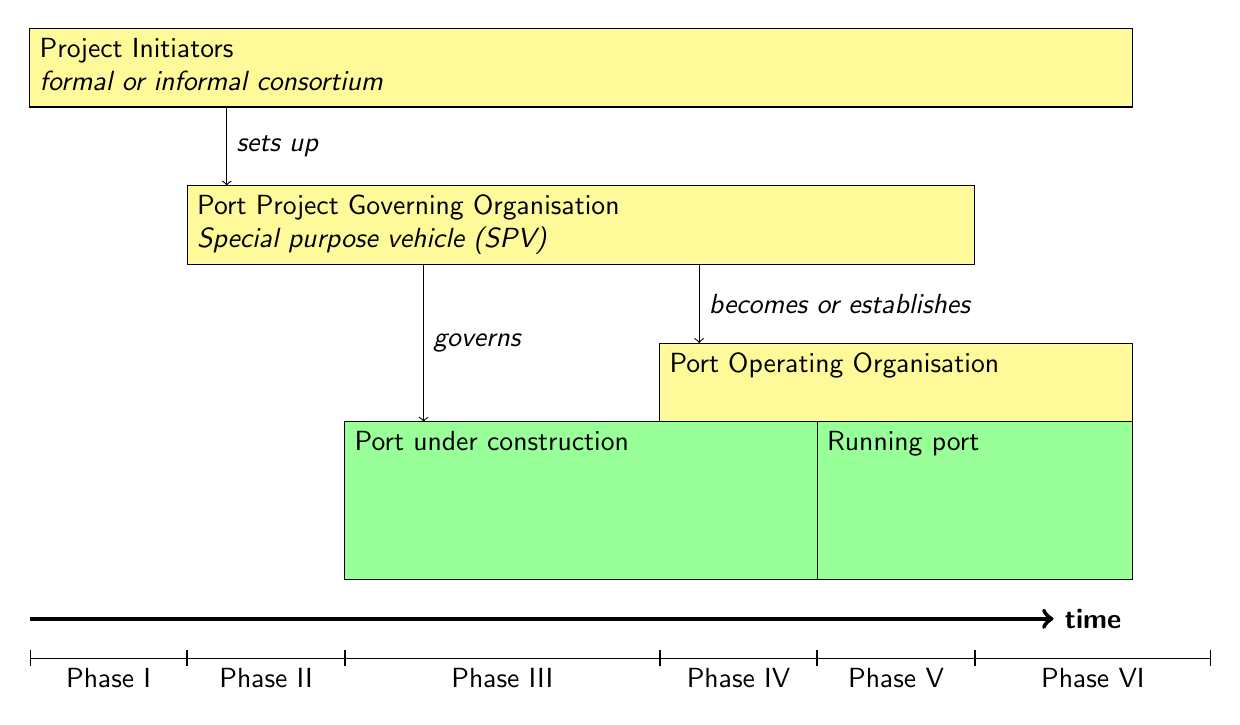
\begin{tikzpicture}

    \tikzset{
        every node/.style={font=\sffamily},
        action/.style={font=\itshape\sffamily},
        myorg/.style={fill=yellow!40},
        myop/.style={fill=green!40}
    }
    
        \draw[myorg] (-2,2) node[below right] {\parbox{12cm}{Project Initiators \\ \textit{formal or informal consortium}}} rectangle (12,1);
        
            \draw[->] (0.5,1) -- node[right,action] {sets up} (0.5,0);
    
        \draw[myorg] (0,0) node[below right] {\parbox{7cm}{Port Project Governing Organisation\\ \textit{Special purpose vehicle (SPV)}}} rectangle (10,-1);
        
            \draw[->] (3,-1) -- node[right,action] {governs} (3,-3);
        
        \draw[myop] (2,-3) node[below right] {Port under construction} rectangle (8,-5);
        
            \draw[->] (6.5,-1) -- node[right,action] {becomes or establishes} (6.5,-2);
        
        \draw[myorg] (6,-2) node[below right] {Port Operating Organisation} rectangle (12,-3);
        \draw[myop] (8,-3) node[below right] {Running port} rectangle (12,-5);
        
        \draw[->,ultra thick] (-2,-5.5) -- (11,-5.5) node[right] {\textbf{time}};
        
        \draw[|-|] (-2,-6) -- node[below] {Phase I} (0,-6);
        
        \draw[|-|] (0,-6) -- node[below] {Phase II} (2,-6);
        
        \draw[|-|] (2,-6) -- node[below] {Phase III} (6,-6);
        
        \draw[|-|] (6,-6) -- node[below] {Phase IV} (8,-6);
        
        \draw[|-|] (8,-6) -- node[below] {Phase V} (10,-6);
        
        \draw[|-|] (10,-6) -- node[below] {Phase VI} (13,-6);

        
    \end{tikzpicture}
    
\end{document}

